\chapter{One-Dimensional Problems} \label{chap:1dim}
We solve the Schrödinger Equation in one-dimensional cases,
\begin{eqnarray}
    \ii \hbar \pp_t \Psi(\vec{r},t) = \hat{H} \Psi(\vec{r},t) \label{eq:time_dependent_schrodinger}
\end{eqnarray}
where $\hat{H} = - \frac{\hbar^2}{2m} \nabla^2 + V(\vec{r},t)$ is the Hamiltonian. 
\section{Stationary cases}
First we consider stationary cases. For stationary, it means $V(\vec{r},t)$ is independent of time. We can use the method of \emph{Separation of Variables}, i.e., 
\begin{eqnarray}
    \wf = \psi(x)\varphi(t)
\end{eqnarray}
then we get the new Schrödinger equation: 
\begin{eqnarray}
    \ii \hbar \frac{1}{\varphi} \frac{\dd \varphi}{\dd t} = - \frac{\hbar^2}{2m} \frac{1}{\psi} \frac{\dd^2 \psi}{\dd x^2} + V
\end{eqnarray}
This means that for \lhs and \rhs are both constant, we denote it as $E$, then we can get two ODEs: 
\begin{align}
   \frac{\dd \varphi}{\dd t} &= - \frac{\ii E}{\hbar} \varphi \label{eq:stationary_time_ode} \\ 
   - \frac{\hbar^2}{2m} \frac{\dd^2 \psi}{\dd x^2} &+ V \psi = E \psi \label{eq:stationary_x_ode}
\end{align}
\cref{eq:stationary_time_ode} is easy to solve: 
\begin{eqnarray}
    \varphi(t) = \ee^{- i E t/ \hbar} \label{eq:time_factor_Schrödinger}
\end{eqnarray}
If we want to solve \cref{eq:stationary_x_ode}, then we need to know $V(x)$. But we can still conclude the general solution: 
\begin{eqnarray}
    \wf = \psi(x) \ee^{- i E t/ \hbar}
\end{eqnarray}
Why we call it stationary? We can check the probability density: 
\begin{eqnarray}
    \abs{\wf}^2 = \wf^* \wf = \psi^* \ee^{+ i E t/ \hbar} \psi \ee^{- i E t/ \hbar} = \abs{\psi(x)}^2
\end{eqnarray}
is independent of time, we can also prove that the mean value of arbitrary observables are also independent of time ($\oO$). \cref{eq:stationary_x_ode} is also called eigenvalue function of energy.

\subsection{Free Particles}
First we consider the most general cases, no absence of external potential, i.e., free particles. \cref{eq:stationary_x_ode} then becomes 
\begin{eqnarray}
    -\frac{\hbar^2}{2m} \frac{\dd^2}{\dd x^2} \psi = E \psi
\end{eqnarray}
or we can also write it as 
\begin{eqnarray}
    \frac{\dd^2}{\dd x^2} \psi + k^2 \psi,\quad k \equiv \frac{2mE}{\hbar} \label{eq:scheq_k}
\end{eqnarray}
The general solution is 
\begin{eqnarray}
    \psi(x) = A \ee^{\ii k x} + B \ee^{- \ii k x}
\end{eqnarray}
To get $A$ and $B$, we need some boundary conditions, but for a free particle, there is no such limits. We directly multiply the time factor obtain in \cref{eq:time_factor_Schrödinger},
\begin{eqnarray}
    \wf = A \exp\left[ik\left(x - \frac{\hbar k}{2m}t\right)\right] + B \exp\left[-ik\left(x + \frac{\hbar k}{2m}t\right)\right] \label{eq:free_general}
\end{eqnarray}
We can also know thatm, for a propagating complex wavefunction we have a general solution in the form below: 
\begin{eqnarray}
    \wf = A \exp\left[i \left(kx - \omega t\right)\right]
\end{eqnarray}
Consider the two terms in \cref{eq:free_general}, the first term as a wave propagating along the $x+$ direction, and the second term as a wave propagating along the $x-$ direction. the only difference is the sign before $k$, if we set 
\begin{eqnarray}
    k \equiv \pm \frac{\sqrt{2 m E}}{\hbar}
\end{eqnarray}
then we can just write \cref{eq:free_general} as 
\begin{eqnarray}
    \wf = A \exp\left[\ii k\left( x - \frac{\hbar k}{2m}t \right)\right]
\end{eqnarray}
Due to de Broglie's formalism $p = \hbar k$, the propagating velocity is 
\begin{eqnarray}
    \omega = \frac{\hbar \abs{k}}{2m} = \sqrt{\frac{E}{2m}}
\end{eqnarray}
Can we still consider $A$ as normalizing the wavefunction? Let's check
\begin{eqnarray}
    \int_{-\infty}^{\infty} \dd x \Psi^* \Psi = \abs{A}^2 \int_{-\infty}^{\infty} \dd x
\end{eqnarray}
The result is divergent. There is no physical meaning of it. How to consider it? Reconsider the \cref{eq:wavefunction_relation_ktox}, which is exactly what we want if multiply the time factor,
\begin{eqnarray}
    \wf = \frac{1}{\sqrt{2 \pi}} \int_{- \infty}^{\infty} \dd k \exp(\ii k\left( x - \frac{\hbar k}{2m}t \right)) \phi_ \alpha(k)
\end{eqnarray}
We find one thing interesting, we didn't announce that this $ k = \pm \sqrt{2mE}/\hbar$ is exactly the momentum, this must be true since 
\begin{eqnarray}
    E = \frac{p^2}{2m}
\end{eqnarray}
is the total energy classicaly, then use the de Broglie formula convert it into quantum energy
\begin{eqnarray}
    E_q = \frac{\hbar^2 k^2}{2m}
\end{eqnarray}
\subsection{1-Dimensional Infinite Potential Well}
Suppose we have potential as \cref{fig:1dwell}
\begin{eqnarray}
    V(x) = \begin{cases}
        0, \quad  0 \leq x \leq a \\
        \infty, \quad \text{else where} 
        \end{cases}
\end{eqnarray}
\begin{figure}[h!]
    \centering
    \begin{tikzpicture}[>=stealth, scale=1]
        \draw[->] (-1,0) -- (5,0) node[right] {$x$};
        \draw[->] (0,0) -- (0,4) node[above] {$V(x)$};
        \draw[thick] (0,3) -- (0,0);    
        \draw[thick] (4,0) -- (4,3);      
        \draw[thick] (0,0) -- (4,0);      
        \node at (2, -0.4) {$0 < x < a$};
        \node at (-0.3, -0.3) {0};
        \node at (4, -0.3) {$a$};
        \node[rotate=90] at (-0.6,2) {$V(x)=\infty$};
        \node[rotate=90] at (4.6,2) {$V(x)=\infty$};
      \end{tikzpicture}
      \caption{1-Dimensional Infinite Potential Well}
      \label{fig:1dwell}
\end{figure}
The particle are free inside the well except the two nodes ($x=0,x=a$). It is impossible to find a particle outside the well, such that the first solution arise.
\begin{eqnarray}
    \psi(x) = 0, \quad x<0 \;\text{or}\; x>a 
\end{eqnarray}
Then inside the well, since potential is 0, \cref{eq:stationary_x_ode} can be written as 
\begin{eqnarray}
    -\frac{\hbar^2}{2m} \frac{\dd^2}{\dd x^2} \psi = E \psi
\end{eqnarray}
Use the same assumption in \cref{eq:scheq_k}, but use different solution assumption,
\begin{eqnarray}
    \psi(x) = A \sin k x + B \cos k x
\end{eqnarray}
The constants depend on the boundary condition. Since the wave function must be continuous, 
\begin{eqnarray}
    \psi(0_+) = \psi(0_-) = 0,\quad \psi(a_-) = \psi(a_+) = 0 
\end{eqnarray}
Such that 
\begin{eqnarray}
    \psi(0_+) = A \sin 0 + B \cos 0 = 0
\end{eqnarray}
and we can know $B = 0$, s.t. 
\begin{eqnarray}
    \psi(x) = A \sin kx
\end{eqnarray}
Therefore 
\begin{eqnarray}
    \psi(a) = A \sin k a = 0
\end{eqnarray}
The constant $A$ can not be zero. So the only condition is 
\begin{eqnarray}
    \sin k a =0 \quad \Ra \quad ka = n \pi, n \in \mathbb{N}
\end{eqnarray}
$k=0$ is also a trivial solution, we can get the final conditoin: 
\begin{eqnarray}
    k_n = \frac{n \pi}{ a}, n \in \mathbb{N}^+
\end{eqnarray}
From this we can get the possible value of $E$, this is exactly the energy of the particle,
\begin{eqnarray}
    E_n = \frac{n^2 \pi^2 \hbar^2}{2m a ^2}
\end{eqnarray}
The possible energy are discrete. Meaning that the quantized particle can only have some definite energies inside the well potential. If we want to know $A$, we then need to normalize the wave function $\psi$: 
\begin{eqnarray}
    \int_{0}^{a} = \abs{A}^2 \sin^2 (kx) \dd x = \abs{A}^2 \frac{a}{2} = 1 
\end{eqnarray}
Solve this we get $A = \sqrt{2/a}$ actually there will be a phase $\ee^{i \theta}$, but we have demenstrate in previous chapter that, a ket multiply a phase factor doesn't change the physics state. And the wave function is the inner product of state ket and position bra. So nothing changed we can just ignore it.
And the final solution of wave function is: 
\begin{eqnarray}
    \psi_n(x) = \sqrt{\frac{2}{a}} \sin \left(\frac{n \pi}{a} x\right)
\end{eqnarray}

\subsection{{Potential Step: Scattering States}} \label{subsec:scattering_state}
Now we consider a time-independent potantial, the wavefunction can be factorized $\wf = \ee^{-\ii Et/\hbar} \psi(x)$, where $\psi(x)$ is obtained from the \cref{eq:stationary_x_ode}. 
\begin{align}
    \frac{\dd^2 \psi}{\dd x^2} = \frac{2m}{\hbar} \left[V(x) - E\right]\psi \label{eq:wavefnction_to_demenstrate_why_continuous_of_dpsi}
\end{align}
Consider a potential step:
\begin{eqnarray}
    V(x) = \begin{cases}
        0, \quad  &x < 0 \\
        V_0, \quad &x > 0
        \end{cases}
\end{eqnarray}
with a finite $V_0$ as shown in \cref{fig:potential_step},
\begin{figure}[h]
    \centering
    \begin{tikzpicture}[scale=1.2]
        % 坐标轴
        \draw[->] (-2,0) -- (2,0) node[right] {$x$};
        \draw[->] (0,-0.5) -- (0,2.5) node[above] {$V(x)$};
      
        % V(x) 的图像
        \draw[thick, black] (-2,0) -- (0,0);
        \draw[thick, black] (0,2) -- (2,2);
        \draw[dashed] (0,0) -- (0,2);
        \node[left] at (0,2) {$V_0$};
      
        % 标注
        \node[below left] at (0,0) {$0$};
      
      \end{tikzpicture}
      \caption{Potential Step in 1-Dimension}
      \label{fig:potential_step}
\end{figure}
The wavefunction $\psi(x)$ and its derivative must be continuous, even the potential is not continuous. Then one may ask, why its first order derivative is necessarily continuous? We look back to \cref{eq:wavefnction_to_demenstrate_why_continuous_of_dpsi}, the $\psi$ denotes a finite wavefunction since $\abs{\psi(x)}^2$ is probability which must be finite. $V(x)$ is also finite in such condition-Potential Step with a finite $V_0$. Such that the \lhs of \cref{eq:wavefnction_to_demenstrate_why_continuous_of_dpsi} is also finite.
\begin{tcolorbox}
   \begin{center}
    $ \frac{\dd^2 \psi}{\dd x^2}$ is bounded $\Ra$ $\psi'(x)$ is continuously differentiable 
   \end{center}
\end{tcolorbox}
If the potential is infinite, z.B. we have a $\delta(x-x')$ potential, which is infinite at $x=x'$, we still disscuss in next subsection \cref{subsec:delta_potential}. Now we continue to disscuss the potential step problem. By solving the \cref{eq:wavefnction_to_demenstrate_why_continuous_of_dpsi}, we get a general solution: 
\begin{alignat}{2}
    \psi_{-}(x) &= \psi_0e^{\ii k x} + r \psi_0 e^{-\ii k_{r} x} \quad && x < 0\label{eq:psi_minus} \\
    \psi_{+}(x) &= t \psi_0 e^{\ii k_{t} x} \quad && x > 0 \label{eq:psi_plus}
\end{alignat}
Actually the general solution can be divided into 3 parts. We consider a wave travel in the x-axis, there is a wall on the path of its propagation, the wave will be reflected by this wall, such that our wave equation would have the solution which is a combination of a incident wave and a reflected wave: 
\begin{alignat}{2}
    \psi_{i}(x) &= \psi_0e^{\ii k x}  \quad && x < 0\label{eq:incident_wave_step} \\
    \psi_{+}(x) &= r\psi_0 e^{-\ii k_{r} x} \quad && x < 0 \label{eq:reflected_wave_step}
\end{alignat}
But this is not a classical condition, the wave can transmit through the wall, such that also a transmitted wave in $x>0$,
\begin{eqnarray}
    \psi_t(x) = t \psi_0 \ee^{\ii k_tx },\quad x>0
\end{eqnarray}
Where the wave vectors of two sign are
\begin{eqnarray}
    k = k_r = \frac{\sqrt{2mE}}{\hbar}, k_t = \frac{\sqrt{\abs{2m(E-V_0)}}}{\hbar}
\end{eqnarray}
We need to disscuss the condition for $k_t$ in different cases, i.e., 
\begin{align}
    k_t = \begin{cases}
        \frac{\sqrt{2m (E-V_0)}}{\hbar}, \quad E>V_0\\
        \frac{\ii \sqrt{2m(V_0-E)}}{\hbar} = \ii \kappa_t, \quad E<V_0
    \end{cases} \label{eq:transmission_wave_vector}
\end{align}
Then we apply the boundar conditions at $x=0$, 
\begin{align}
    \psi_i(0) + \psi_r(0) &= \psi_t(0)\quad \rightleftarrows \quad 1 + r = t\\
    \psi'_i(0) + \psi'_r(0) &= \psi'_t(0)\quad \rightleftarrows \quad \ii k(1-r) = \ii k_t r 
\end{align}
By this we can find the relection and transmission amplitudes,
\begin{align}
    r &= \frac{k - k_t}{k + k_t} =  \frac{\sqrt{E} - \sqrt{E - V_0}}{\sqrt{E} + \sqrt{E - V_0}}\; \text{or}\; \frac{\sqrt{E} - \ii \sqrt{V_0 - E}}{\sqrt{E} +\ii \sqrt{V_0 - E}} \quad \text{(reflection amplitude)} \label{eq:reflection_amplitude} \\
    t &= 1 + r = \frac{2k}{k + k_t} = \frac{2 \sqrt{E}}{\sqrt{E} + \sqrt{E - V_0}} \text{or} \frac{2 \sqrt{E}}{\sqrt{E} +\ii \sqrt{V_0 - E}}\quad \text{(transmission amplitude)} \label{eq:transmission_amplitude}
\end{align}

Now we consider different conditions as we mentioned in: 
\begin{enumerate}
    \item $E > V_0:\quad k_t \in \R$ \\
    Then, two different conditions need to be disscuss when considering \cref{eq:reflection_amplitude}, 
    \begin{itemize}
        \item $V_0>0: \quad r,t >0$ \\
        There is no phase difference between incident wave and reflection wave, such that we can conclude the two waves are in phase, as shown in \cref{fig:scatter_inphase}.
        \begin{figure}[h!]
            \centering
            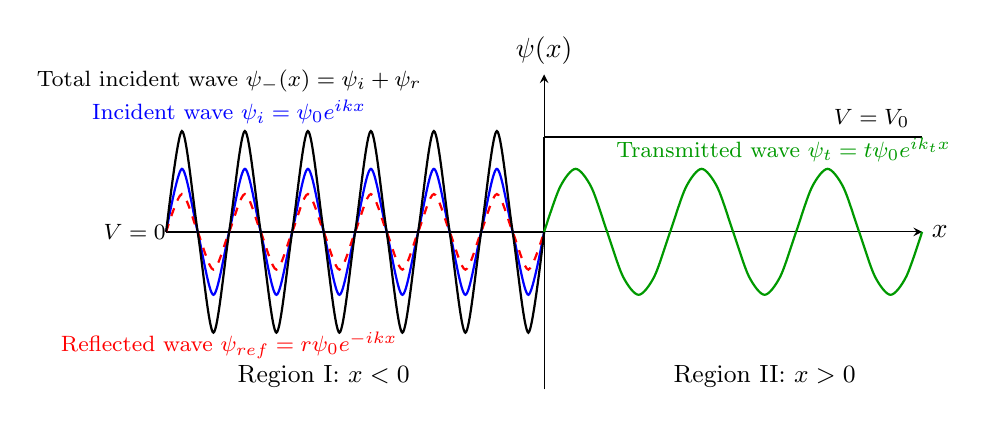
\begin{tikzpicture}[scale=0.8, >=stealth]

                % Axes
                \draw[->] (-6,0) -- (6,0) node[right] {$x$};
                \draw[->] (0,-2.5) -- (0,2.5) node[above] {$\psi(x)$};
                
              
                % Potential step shape (above x-axis)
                \draw[thick] (-6,0) -- (0,0); % left constant
                \draw[thick] (0,0) -- (0,1.5); % vertical step line, for clarity
                \draw[thick] (0,1.5) -- (6,1.5); % right lower step
                \node at (-6.5,0) {\footnotesize $V = 0$};
                \node at (5.2,1.8) {\footnotesize $V = V_0$};
              
                % Incoming wave (blue)
                \draw[domain=-6:0, smooth, thick, blue] plot (\x, {sin(deg(2*pi*\x))});
                \node[blue] at (-5,1.9) {\footnotesize Incident wave $\psi_i = \psi_0 e^{ikx}$};
              
                % Reflected wave (red)
                \draw[domain=-6:0, smooth, thick, red, dashed] plot (\x, {0.6*sin(deg(2*pi*\x))});
                \node[red] at (-5,-1.8) {\footnotesize Reflected wave $\psi_{\text{ref}} = r \psi_0 e^{-ikx}$};
              
                % Total wave (black)
                \draw[domain=-6:0, smooth, thick, black] plot (\x, {sin(deg(2*pi*\x)) + 0.6*sin(deg(2*pi*\x))});
                \node[black] at (-5,2.4) {\footnotesize Total incident wave $\psi_-(x) = \psi_{i} + \psi_{r}$};
              
                % Transmitted wave (green)
                \draw[domain=0:6, smooth, thick, green!60!black] plot (\x, {sin(deg(pi*\x))});
                \node[green!60!black] at (3.8,1.3) {\footnotesize Transmitted wave $\psi_{t} = t \psi_0 e^{ik_t x}$};
              
                % Region labels
                \node at (-3.5,-2.3) {\small Region I: $x < 0$};
                \node at (3.5,-2.3) {\small Region II: $x > 0$};
              
              \end{tikzpicture}
              \caption{$\text { Potential step scattering with } E>V_0 \text { and } V_0>0$}
              \label{fig:scatter_inphase}
        \end{figure}

        one can prove that although the wave function is non-normalized, the total probability total \cref{eq:probability_current} is conserved. First give the three currents of different waves: 
        \begin{align}
            j_i &= \frac{\hbar k}{m} \abs{\psi_0}^2 \\
            j_r &= - \frac{\hbar k}{m} \abs{r}^2 \abs{\psi_0}^2 \\
            j_t &= \frac{\hbar k_t}{m} \abs{t}^2 \abs{\psi_0}^2
        \end{align}
        Then, calculate the total incident probability current and compare this with transmitted probability current,
        \begin{align}
            j_i + j_r &= \frac{\hbar k}{m} \left(1- \abs{r}^2\right) \abs{\psi}^2 = \frac{\hbar k}{m} \frac{4 k k_t}{(k+k_t)^2} \abs{\psi_0}^2 \\
            j_t &= \frac{\hbar k_t}{m} \frac{4k^2}{(k+k_t)^2} \abs{\psi}^2 = j_i+j_r
        \end{align}
        \item $V_0<0: \quad r<0,t>0$\\
        The reflected wave has a phase jump\footnote{which also called a scattering phase} $\delta=\pi$, as shown in \cref{fig:scatter_outphase}. The phase jump comes from our result $r = - \abs{r}$, the condition for current conservation is exactly as same as disscussed above.
        \begin{figure}[h!]
            \centering
            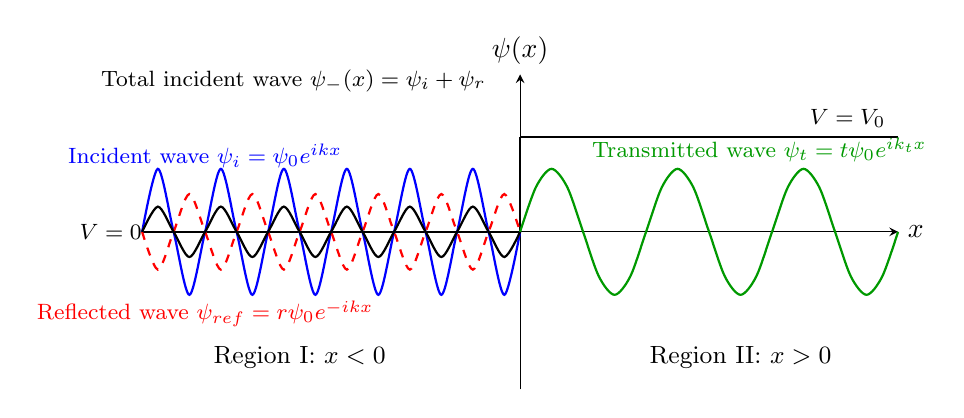
\begin{tikzpicture}[scale=0.8, >=stealth]

                % Axes
                \draw[->] (-6,0) -- (6,0) node[right] {$x$};
                \draw[->] (0,-2.5) -- (0,2.5) node[above] {$\psi(x)$};
                
              
                % Potential step shape (above x-axis)
                \draw[thick] (-6,0) -- (0,0); % left constant
                \draw[thick] (0,0) -- (0,1.5); % vertical step line, for clarity
                \draw[thick] (0,1.5) -- (6,1.5); % right lower step
                \node at (-6.5,0) {\footnotesize $V = 0$};
                \node at (5.2,1.8) {\footnotesize $V = V_0$};
              
                % Incoming wave (blue)
                \draw[domain=-6:0, smooth, thick, blue] plot (\x, {sin(deg(2*pi*\x))});
                \node[blue] at (-5,1.2) {\footnotesize Incident wave $\psi_i = \psi_0 e^{ikx}$};
              
                % Reflected wave (red)
                \draw[domain=-6:0, smooth, thick, red, dashed] plot (\x, {0.6*sin(deg(-2*pi*\x))});
                \node[red] at (-5,-1.3) {\footnotesize Reflected wave $\psi_{\text{ref}} = r \psi_0 e^{-ikx}$};
              
                % Total wave (black)
                \draw[domain=-6:0, smooth, thick, black] plot (\x, {sin(deg(2*pi*\x)) + 0.6*sin(deg(-2*pi*\x))});
                \node[black] at (-3.6,2.4) {\footnotesize Total incident wave $\psi_-(x) = \psi_{i} + \psi_{r}$};
              
                % Transmitted wave (green)
                \draw[domain=0:6, smooth, thick, green!60!black] plot (\x, {sin(deg(pi*\x))});
                \node[green!60!black] at (3.8,1.3) {\footnotesize Transmitted wave $\psi_{t} = t \psi_0 e^{ik_t x}$};
              
                % Region labels
                \node at (-3.5,-2) {\small Region I: $x < 0$};
                \node at (3.5,-2) {\small Region II: $x > 0$};
              
              \end{tikzpicture}
              \caption{$\text { Potential step scattering with } E>V_0 \text { and } V_0<0$}
              \label{fig:scatter_outphase}
        \end{figure}
    \end{itemize}
    \item $E<V_0: \quad k_t = \ii \kappa_t, \; \kappa_t \in \R$, in such case, we can write the wavefunction as 
    \begin{eqnarray}
        \psi_t(x) = t \psi_0 \ee^{\kappa_t x} 
    \end{eqnarray}
    \begin{figure}[h]
        \centering
        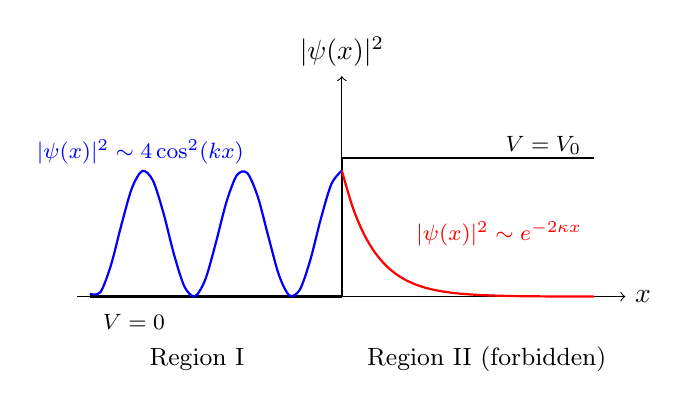
\begin{tikzpicture}[scale=0.8]

    % Define constants
    \def\k{2}          % wave number k
    \def\kk{1}         % decay rate kappa
  
    % Axes
    \draw[->] (-4.2,0) -- (4.5,0) node[right] {$x$};
    \draw[->] (0,0) -- (0,3.5) node[above] {$|\psi(x)|^2$};
  
    % Potential step
    \draw[thick] (-4,0) -- (0,0);     % left side flat
    \draw[thick] (0,0) -- (0,2.2);    % drop
    \draw[thick] (0,2.2) -- (4,2.2);  % right side flat
    \node at (-3.3,-0.4) {\footnotesize $V = 0$};
    \node at (3.2,2.4) {\footnotesize $V = V_0$};
  
    % Vertical dashed line at x=0
    \draw[dashed] (0,0) -- (0,3.2);
  
    % Region labels
    \node at (-2.3,-1) {\small Region I};
    \node at (2.3,-1) {\small Region II (forbidden)};
  
    % Left side: cosine squared wave (standing wave)
    \draw[domain=-4:0, smooth, thick, blue]
      plot (\x, {2*(cos(deg(\k*\x)))^2});
  
    % Right side: exponential decay
    \draw[domain=0:4, smooth, thick, red]
      plot (\x, {2*exp(-2*\kk*\x)});
  
    % Labels
    \node[blue] at (-3.2,2.3) {\footnotesize $|\psi(x)|^2 \sim 4\cos^2(kx)$};
    \node[red] at (2.5,1) {\footnotesize $|\psi(x)|^2 \sim e^{-2\kappa x}$};
  
        \end{tikzpicture}
        \caption{Potential step scattering with $E<V_0$}
        \label{fig:scattering_forbidden}
    \end{figure}
    Now our amplitudes are not real numbers, we can not give it a physical explainations. But if we look at the reflected amplitude, the $\abs{r}^2$ denotes the reflection probability, we can calculate it 
    \begin{eqnarray}
        R = \abs{r}^2 = \abs{\frac{k - \ii \kappa_t}{k + \ii \kappa_t}}^2 = 1
    \end{eqnarray}
    The incident wave reflected completely! There should be no transmitted wave! Now a new question arise, why $\psi_t(x)$ is non-zero expcet $x \ra + \infty$? This means the particle penetrate into the barrier, which is calssical forbidden, but do not propagate. The result is as shown in \cref{fig:scattering_forbidden}.
\end{enumerate}
\subsection{\texorpdfstring{$\delta$}{delta} Function Potential} \label{subsec:delta_potential}




\subsection{1-Dimensional Finite Potential Well: Bounded States}

At \cref{subsec:scattering_state} we disscussed the scattering states, which means that, after the wave incident the potential barrier, the wave was scattered by this potential. Since it is just a one dimensional case, the scattering wave can not behave like the behavior as Compton Scattering in 3-d world. Now we consider a finite potential well to study the bounded state, we will explain what does it mean after we get the full result.

Following the given potential, also as shown in 
\begin{eqnarray}
    V(x) = \begin{cases}
        0, \quad  &0<x<a\\
        V_0, \quad &\mathrm{others}
        \end{cases}
\end{eqnarray}

\begin{figure}[h!]
    \centering
    \begin{tikzpicture}[scale=0.8]
        \draw[->] (-3,0) -- (6,0) node[right] {$x$};
        \draw[->] (0,0) -- (0,4) node[above] {$V(x)$};

        \draw[thick] (-3,3) -- (0,3);
        \draw[thick] (0,0) -- (3,0);
        \draw[thick] (3,3) -- (6,3);
        \draw[thin] (3,0) -- (3,3);
        \node at (1.1,0.4) {\footnotesize $V = 0$};
        \node at (4.1,3.4) {\footnotesize $V = V_0$};
        \node at (-1.1,3.4) {\footnotesize $V = V_0$};
    \end{tikzpicture}
    \caption{The finite potential well}
    \label{fig:finite_potential_well}
\end{figure}

Recall the SE \cref{eq:stationary_x_ode} we get 
\begin{eqnarray}
    \frac{\dd^2 \psi}{\dd x^2} = \frac{2m}{\hbar} \left[ V(x) - E \right] \psi
\end{eqnarray}

As we already disscussed in last section, we need to consider the relation between energy of the particle and the potential, also in following form 
\begin{align}
    k = \begin{cases}
        \frac{\sqrt{2m(E - V_0)}}{\hbar}, \quad E> V_0 \\
        \frac{\ii\sqrt{2m(V_0 - E)}}{\hbar}, \quad E< V_0
    \end{cases}
\end{align}


\newpage
\section{1-Dimensional Harmonic Oscillators: Extension of Hilbert Space}
We condsider the Hamiltonian of a Harmonic Oscillator calssically, 
\begin{eqnarray}
    H = \frac{p^2}{2m} + \frac{1}{2} m \omega^2 x^2
\end{eqnarray}
then move to a quantum condition, i.e., $p \ra \op, x \ra \ox$, and we get the Hamiltonian Operator,
\begin{eqnarray}
    \oH = \frac{\op^2}{2m} + \frac{1}{2} m \omega^2 \ox^2
\end{eqnarray}
The Hamiltonian of Harmonic Oscillator is time-independent and Hermitian, due to \cref{eq:stationary_x_ode,theorem:spectrum_hermitian}, such kind of condition would have a energy eigenvalue function: 
\begin{align}
    \oH \ket{\psi_ \nu^i} = E_ \nu \ket{\psi_ \nu^i} \label{eq:SHO_eigenvalue_equation}
\end{align}
Here we won't study the general wave function in a definite representation, we will talk about it later as we finish the eigenvector and eigenvalue problems. 

\subsection{Eigenvalues of the Hamiltonian}
First we extend our operators $\ox,\op$ to such form: 
\begin{align}
    \oX &= \sqrt{\frac{m \omega}{\hbar}} \ox \\
    \oP &= \frac{1}{\sqrt{m \hbar \omega}} \op
\end{align}
The new commutator is 
\begin{align}
    \comm{\oX}{\oP} = \sqrt{\frac{m \omega}{\hbar}} \cdot \frac{1}{\sqrt{m \hbar \omega}} \comm{\ox}{\op} = \frac{1}{\hbar} \ii \hbar = \ii
\end{align}
Now the Hamiltonian becomes
\begin{align}
    \oH = \frac{\hbar \omega}{2} \left(\oX^2 + \oP^2\right) \label{eq:Hamiltonian_SHO_xp}
\end{align}
Now we shall explain why we construct such a form, since the observables obviously have dimensions\footnote{$\ox:[\mathrm{m}],\op:[\mathrm{m \cdot kg \cdot s^{-1}}]$}. The dimension of $\hbar$ is $[\mathrm{m^2 \cdot kg \cdot s^{-1}}]$, the dimension of $\omega$ is $[\mathrm{s^{-1}}]$, it is easy to see that the new operators have same dimension as we wish.

Now we study more about the new operators, we find the fact $\oX^2 + \oP^2 = \left(\oX - \ii \oP\right) \left(\oX + \ii \oP\right)$, therefor we set, 
\begin{align}
    \a &= \frac{1}{\sqrt{2}} \left(\oX + \ii \oP\right) = \frac{1}{\sqrt{2}} \left( \sqrt{\frac{m \omega}{\hbar}} \ox + \ii \frac{1}{\sqrt{m \hbar \omega}} \op \right)\\
    \adag & = \frac{1}{\sqrt{2}} \left(\oX - \ii \oP\right) = \frac{1}{\sqrt{2}} \left( \sqrt{\frac{m \omega}{\hbar}} \ox - \ii \frac{1}{\sqrt{m \hbar \omega}} \op \right)
\end{align}
Inversly,
\begin{align}
    \ox = \sqrt{\frac{\hbar}{2m\omega}} \left(\adag+ \a\right) \label{eq:ox_as_aadag} \\ 
    \op = \ii \sqrt{\frac{m \hbar \omega}{2}} \left(\adag - \a\right) \label{eq:op_as_aadag}
\end{align}
We can compute the commutator of $\a,\adag$, 
\begin{eqnarray}
    \comm{\a}{\adag} = \frac{1}{2} \comm{\oX + \ii \oP}{\oX + \ii \oP} = \frac{\ii}{2} \comm{\oP}{\oX} - \frac{\ii}{2} \comm{\oX}{\oP} = -\frac{ \ii}{2} \times \ii \times 2 = 1
\end{eqnarray}
Thus we obtain an important relation,
\begin{eqnarray}
    \a \adag = 1 + \adag \a 
\end{eqnarray}
The last term of \rhs is 
\begin{align}
    \adag \a = \frac{1}{2} \left(\oX - \ii \oP\right) \left( \ox + \ii \oP \right) &= \frac{1}{2} \left[\oX^2 + \ii\left( \oX \oP - \oP \oX \right) + \oP^2 \right] = \frac{1}{2} \left( \oX^2 + \oP^2 -1 \right) \\
    &= \frac{1}{2} \left(\oX^2+ \oP^2 + \ii \comm{\oX}{\oP}\right) = \frac{1}{2} = \left(\oX^2 + \oP^2 -1\right) 
\end{align}
Reconsider \cref{eq:Hamiltonian_SHO_xp}, using the result above, we obtain
\begin{align}
    \oH = \hbar \omega \left(\adag \a + \frac{1}{2}\right) = \hbar \omega \left( \a \adag - \frac{1}{2} \right) \label{eq:Hamiltonian_SHO_aadag}
\end{align}
We define a new operator\footnote{Also called Number Operator} as
\begin{align}
    \widehat{N} := \adag \a \label{eq:number_operator}
\end{align}
Now the Hamiltonian becomes,
\begin{align}
    \oH = \hbar \omega \left( \oN + \frac{1}{2} \right)\label{eq:Hamiltonian_SHO_number}
\end{align}
So the eigenvectors of Hamiltonian are definitly the eigenvectors of $\oN$. Before we get to the eigenvectors and eigenvalues, we want also disscuss the commutators related, 
\begin{align}
    \comm{\a}{\a} = \frac{1}{2} \comm{\oX + \ii \oP}{\oX - \ii \oP} = \frac{\ii}{2} \left(\comm{\oX}{\oP} + \comm{\oP}{\oX}\right) = 0 \\
    \comm{\adag}{\adag} = \frac{1}{2} \comm{\oX - \ii \oP}{\oX + \ii \oP} = \frac{\ii}{2} \left(\comm{\oX}{\oP} + \comm{\oP}{\oX}\right) = 0
\end{align}
And also 
\begin{align}
    \comm{\oN}{\a} &= \comm{\adag \a}{\a} = \adag \comm{\a}{\a} + \comm{\adag}{\a} \a = 0 - \a = \a \\
    \comm{\oN}{\adag} &= \comm{\adag \a}{\adag} = \adag \comm{\a}{\adag} + \comm{\adag}{\adag} \a = \adag + 0 = \adag
\end{align}
By \cref{eq:Hamiltonian_SHO_number} we obtain, 
\begin{align}
    \comm{\oH}{\a} = - \hbar \omega \a \\
    \comm{\oH}{\adag} = \hbar \omega \adag
\end{align}
We could define the eigenvalue equation of number state 
\begin{eqnarray}
    \oN \ket{\psi_ \nu^ i} =  \nu\ket{\psi_ \nu^i}
\end{eqnarray}
The eigenvalue equation \cref{eq:SHO_eigenvalue_equation} also, 
\begin{eqnarray}
    \oH \ket{\psi_ \nu ^i} = \left( \nu + \frac{1}{2}\right) \ket{\psi_ \nu^i} 
\end{eqnarray}
Now we study the properties of the eigenvalues and eigenvectors of $\oN$.
\subsubsection{Determination of the Spectrum}
First we disscuss the properties of eigenvalues of $\oN$. We follow a lemma–proof structure to carry out the analysis,
\begin{lemma} \label{lemma:SHO_eigenvalue_nonnegative}
    The Eigenvalues $ \nu$ of the operator $\oN$ are non-negative.
\end{lemma}
\begin{proof}
    Consider an arbitrary eigenvector $\ket{\psi_ \nu^i}$ of $\oN$. Consider the square of norm of the vector $\a \ket{\psi_ \nu^i}$ is non-negative,
    \begin{eqnarray}
        \norm{\a \ketsho}^2 = \brasho \adag \a \ketsho \geq 0
    \end{eqnarray}
    the operator in front of the bra ket is just the number operator. Now, the square of norm is
    \begin{eqnarray}
        \brasho \oN \ketsho = \brasho \nu \ketsho = \nu \braket{\psi_ \nu^i|\psi_ \nu^i} \label{eq:SHO_eigenvalue_norm}
    \end{eqnarray}
    The norm $\braket{\psi_ \nu^i|\psi_ \nu^i}$ is positive. Such that the eigenvalues $\nu \geq 0$
\end{proof}

\begin{lemma} \label{lemma:annihilation_properties}
    Let $\ketsho$ be a (non-zero) eigenvector of $\oN$ with the eigenvalue $\nu$ 
    \begin{enumerate}
        \item If $ \nu = 0$, the ket $\a \ket{\psi_{\nu=0}^i}$ is zero. 
        \item If $ \nu > 0$, the ket $\a \ketsho$ is a non-zero eigenvector of $\oN$ with the eigenvalue $ \nu -1 $
    \end{enumerate}
\end{lemma}

\begin{proof}
    \begin{enumerate}
        \item According to \cref{eq:SHO_eigenvalue_norm}, if $ \nu=0$, $\norm{\ketsho}$ is zero vector. Such that $\nu =0 $ is the eigenvalue of $\oN$, the following holds:
        \begin{eqnarray}
            \a \ket{\psi_0^i} = 0
        \end{eqnarray}
        \item Consider the vector $\a \ket{\psi_ \nu^i}$
        \begin{align}
            \a \ket{\psi_ \nu^i} =& - \comm{\oN}{\a} \ketsho = \a \oN \ketsho - \oN \a \ketsho \notag \\
            =&  \nu \a \ketsho - \oN \a \ketsho \notag \\
            \Ra& \oN \a \ketsho = \left( \nu - 1\right) \a \ketsho
        \end{align}
    \end{enumerate}
\end{proof}

\begin{lemma} \label{lemma:creation_properties}
    Let $\ketsho$ be a (non-zero) eigenvector of $\oN$ of eigenvalue $\nu$, the followings are true 
    \begin{enumerate}
        \item $\adag \ketsho$ is always non-zero. 
        \item $\adag \ketsho$ is an eigenvector of $\oN$ with the eigenvalue $\nu + 1$
    \end{enumerate}
\end{lemma}

\begin{proof}
    \begin{enumerate}
        \item The norm of $\adag \ketsho$ is 
        \begin{align}
            \norm{\adag \ketsho}^2 &= \brasho \a \adag \ketsho \notag \\
            &= \brasho (\adag \a + 1) \ketsho \notag \\ 
            &= \brasho \left(\oN + 1\right) \ketsho \notag \\
            &= \left(\nu + 1\right) \braket{\psi_ \nu^i| \psi_ \nu^i}
        \end{align}
        Due to \cref{lemma:SHO_eigenvalue_nonnegative}, the ket $\adag \ketsho$ always has a non-zero norm and, consequently, is never zero. 
        \item Consider the vector $\adag \ketsho$ 
        \begin{align}
            \adag \ketsho &= \comm{\oN}{\adag} \ketsho = \oN \adag \ketsho - \adag \oN \ketsho \notag \\
            &= \oN \adag \ketsho -  \nu \adag \ketsho \notag \\
            \Ra& \oN \adag \ketsho = \left( \nu + 1\right) \ketsho
        \end{align}
    \end{enumerate}
\end{proof}

Then, we use lemmas above to give the fact that the spectrum of $\oN$ is composed of non-negative integers. We use proof by contradiction, we suppose $ \nu$ is non-integer we can always find an integer $n \geq 0$ such that: 
\begin{eqnarray} 
    n <  \nu < n+1 \label{eq:SHO_hypothesis}
\end{eqnarray}
we can consider a series of vectors, 
\begin{eqnarray}
    \ketsho, \a \ketsho, \dots, \a^n \ketsho
\end{eqnarray}
if we have the p-th vector in this series, this must be non-zero, and its corresponding eigenvalue is $\nu -p$. This is easy to prove by iteration, we won't give the details. But it is true. We now consider the $\a^ n \ketsho$, its corresponding eigenvalue $ \nu - n$, and this is a non-zero vector. Again, $\a^ {n+1} \ketsho$, the corresponding eigenvalue of this ket is $\nu - n - 1$, this should be positive as our \cref{lemma:annihilation_properties}, but as our hypothesis \cref{eq:SHO_hypothesis}, this should be strictly negative. Since they contract each other, we can convince that $\nu$ is integer. As we have defined $\nu$ belongs to a index set. So we can now write it as just $\nu$. Due to \cref{lemma:creation_properties}, the spectrum $\oN$ indeed includes all positive and zero integers. From this we can see check the eigenvalue of $\oH$ again, this should be 
\begin{eqnarray}
    E_n = \left(n+ \frac{1}{2}\right) \hbar \omega
\end{eqnarray}
We could find the energy of the Harmonic Oscillator is quantized and cannot take on any arbirtay value. The ground state now is not 0, but $\hbar \omega/2$.

\subsubsection{Degenracy of the eigenvalue}
When we talking about the eigenvalues of an Operator, it is essential to talk about the degenracy. 

The eigenvectors of $\H$ associated with the eigenvalue $E_0 \hbar \omega/2$, which is, the eigenvectors of $\oN$ associated with the eigenvalue $n=0$, must satisfy the equation: 
\begin{eqnarray}
    \a \ket{\psi_0 ^i} = 0
\end{eqnarray}
To find the degenracy of the ground state, all we must do is see how many linearly independent kets satisfy the equation above. Expand this as 
\begin{eqnarray}
    \frac{1}{\sqrt{2}} \left( \sqrt{\frac{m \omega}{\hbar}} \ox + \frac{\ii}{\sqrt{m \hbar \omega}}\op \right) \ket{\psi_0 ^i} = 0
\end{eqnarray}
Write it in the position representation, this relation becomes: 
\begin{eqnarray}
    \left(\frac{m\omega}{\hbar}\ox + \frac{\dd}{\dd x}\right) \psi_0^i(x) = 0
\end{eqnarray}
The general solution is 
\begin{eqnarray}
    \psi_0^i (x) = A \exp\left(- \frac{1}{2} \frac{m \omega}{\hbar} x^2\right)
\end{eqnarray}
This means the solutions of the equation are propotional to the exponential term. Such that there are no more kets satisfy the differential equation: the ground state is not degenerate. 
Now we check the other states, all what we need to prove is that, if the level $E_n = (n + 1/2)\hbar \omega$ is not degenerate, the level $E_{n+1} = (n+1 + 1/2)\hbar \omega$ is not either, i.e., 
\begin{eqnarray}
    \oN \ketshoizero = n \ketshoizero
\end{eqnarray} 


\subsection{Eigenvectors of the Hamiltonian}
The vector $\ket{\psi_0}$ associated with $n=0$ is the vector which satisfy:
\begin{eqnarray}
    \a \ket{\psi_0} = 0
\end{eqnarray}
It is defined to within a constant factor; we shall assume this is normalized. And it is propotional to $\ket{\psi_1}$,
\begin{eqnarray}
    \ket{\psi_1} = c_1 \adag \ket{\psi_0}
\end{eqnarray}
this is also normalized
\begin{eqnarray}
    \braket{\psi_1|\psi_1} = c_1^* c_1 \bra{\psi_0} \a \adag \ket{\psi_0} = \abs{c_1}^2 \bra{\psi_0} (\adag \a + 1) \ket{\psi_0} = \abs{c_1}^2 =1 
\end{eqnarray}
Such that 
\begin{eqnarray}
    \ket{\psi_1} = \adag \ket{\psi_0}
\end{eqnarray}
similarly we can prove the following: 
\begin{eqnarray}
    \ket{\psi_n} = \frac{1}{\sqrt{n}} (\adag)^n \ket{\psi_0} 
\end{eqnarray}
This just relate some trivial calculation. Won't give it explicitly here.
\subsubsection{Orthonormalization and closure relations}
Since $\H$ is Hermitian, the spectrum of it must consist of a set of eigenvectors which are orthonormal, i.e.
\begin{eqnarray}
    \braket{\psi'_n|\psi_n} = \delta_{n'n}
\end{eqnarray}
Also they are complete sets 
\begin{eqnarray}
    \sum_n \ket{\psi_n} \bra{\psi_n} = \I
\end{eqnarray}
Now we rewrite $\ket{\psi_n} = \ket{n}$, $n$ contains every information we need, we don't need to use $\psi$ to denote it anymore.

\subsubsection{Creation and Annihilation Operators on the eigenvectors}
In the basis of $\basispsi$, the action of the creation and annihilation operators on the kets is given by, 
\begin{align}
    \adag \ket{n} = \sqrt{n} \ket{n+1} \label{eq:Creation_eigenequation} \\
    \a \ket{n} = \sqrt{n} \ket{n-1} \label{eq:Annihilation_eigenequation}
\end{align}
Now we explain, why we call them Creation ($\adag$) and Annihilation ($\a$) Operators, \cref{eq:Creation_eigenequation} shows the creation operator can raise $n$ to $n+1$, like it creates a particle, \cref{eq:Annihilation_eigenequation} shows the annihilation operator can lower $n$ to $n-1$, like it annihilation a particle. 

What is eigenvalue of $\ox$ and $\op$? Using
\begin{eqnarray}
    \ox \ket{n} = \sqrt{\frac{\hbar}{2m \omega}} \left(\adag + \a\right) \ket n = \sqrt{\frac{\hbar}{2m \omega}} \left[\sqrt{n+1}\ket{n+1} + \sqrt{n} \ket{n-1}\right] \\
    \op \ket n = \ii \sqrt{\frac{m \hbar \omega}{2}} \left(\adag - \a\right) \ket n = \ii \sqrt{\frac{m\hbar \omega}{2}} \left[ \sqrt{n+1} \ket{n+1} - \sqrt{n} \ket{n-1} \right]
\end{eqnarray}
Now consider the wavefunction of the state, in position representation, i.e., $\braket{x|n} = \psi_n(x)$, 
\begin{eqnarray} 
    \bra{x} \ox \ket{n} = x \psi_n(x) = \sqrt{\frac{\hbar}{2m \omega}} \left( \sqrt{n+1} \psi_{n+1}(x) + \sqrt{n} \psi_{n-1}(x) \right) \\ 
    \bra{x} \op \ket{n} = - \ii \hbar \frac{\dd}{\dd x} \psi_n(x) = \ii \sqrt{\frac{m \hbar \omega}{2}} \left( \sqrt{n+1} \psi_{n+1}(x) - \sqrt{n} \psi_{n-1}(x) \right)
\end{eqnarray}
Now set $\xi = \sqrt{m \omega/\hbar}x, \alpha = \sqrt{\hbar/ 2m\omega}$. Plug in these into the equation above, we obtain: 
\begin{align*}
    &\sqrt{\frac{\hbar}{m \omega}}\xi \psi_n(\xi) = \sqrt{\frac{\hbar}{2m \omega}} \left( \sqrt{n+1} \psi_{n+1}(\xi) + \sqrt{n} \psi_{n-1}(\xi) \right) \\ 
    \Ra\quad& \xi \psi_n(\xi) = \frac{1}{\sqrt{2}} \left( \sqrt{n+1} \psi_{n+1}(\xi) + \sqrt{n} \psi_{n-1}(\xi) \right) \label{eq:xi_psin} \numberthis \\ 
    & -\sqrt{ m \omega \hbar} \frac{\dd}{\dd \xi}  \psi_n(\xi) = \sqrt{\frac{m \hbar \omega}{2}} \left( \sqrt{n+1} \psi_{n+1}(\xi) - \sqrt{n} \psi_{n-1}(\xi) \right) \\
    \Ra \quad& \psi'_n(\xi) = \frac{1}{\sqrt{2}} \left( \sqrt{n+1} \psi_{n+1}(\xi) - \sqrt{n} \psi_{n-1}(\xi) \right) \label{eq:psin_diff} \numberthis
\end{align*} 
We sum and subtract \cref{eq:xi_psin,eq:psin_diff} and obtain, 
\begin{eqnarray}
    &\psi'_n(\xi) + \xi \psi_n(\xi) - \sqrt{2} \sqrt{n+1} \psi_{n+1}(\xi) = 0 \\
    &\psi'_n(\xi) - \xi \psi_n(\xi) + \sqrt{2} \sqrt{n} \psi_{n-1}(\xi) = 0
\end{eqnarray}
Now we investigate the ground state and first several excited states by using \cref{eq:Creation_eigenequation,eq:Annihilation_eigenequation}
\begin{align*}
    & \bra{x} \a \ket{0} = \frac{1}{\sqrt{2}} \left( \sqrt{\frac{m \omega}{\hbar}}\ox + \ii \frac{1}{\sqrt{m \hbar \omega}} \op \right) \psi_0(x) = 0 \\
    \Ra \quad&\frac{m \omega}{\hbar} x + \frac{\dd}{\dd x} \psi_0(x) = 0 \Ra \psi_0(x) = A \exp\left(-\frac{m \omega }{2 \hbar} x^2\right)
\end{align*}
Now we normalize this 
\begin{eqnarray}
    1 = \int_{-\infty}^{\infty} \dd x \abs{\psi_0(x)}^2 = \abs{A}^2 \int_{-\infty}^{\infty} \dd x \exp\left(-\frac{m \omega }{2 \hbar} x^2\right) = A^2 \sqrt{\frac{\hbar \pi}{m \omega}} \quad \Ra \quad A = \left(\frac{m \omega}{\pi \hbar}\right)^{1/4}
\end{eqnarray}
Also we can also obtain the first and second excited state $\psi_1 = \braket{x|1}, \psi_1 = \braket{x|2}$
\begin{align*}
    \braket{x|1} = \bra{x}\adag \ket{0} = \frac{1}{\sqrt{2}} \left( \sqrt{\frac{m \omega}{\hbar}} x - \ii \frac{1}{\sqrt{m \hbar \omega}} \left(- \ii \hbar \frac{\dd}{\dd x}\right) \right) \psi_0(x) \\
    \braket{x|2} = \frac{1}{\sqrt{2!}}\bra{x}{(\adag)}^2\ket{0} = \frac{1}{\sqrt{2}} \left( \sqrt{\frac{m \omega}{\hbar}} x - \ii \frac{1}{\sqrt{m \hbar \omega}} \left(- \ii \hbar \frac{\dd}{\dd x}\right) \right)^2 \psi_0(x)
\end{align*}
Plug in $\psi_0$ into above, one can obtain, 
\begin{align}
    \psi_1(x) = \sqrt{\frac{2 m \omega}{\hbar}} x \psi_0(x) = \sqrt{\frac{2}{\sqrt{\pi}}} \left(\frac{m \omega}{\hbar}\right)^{3/4}x \exp \left(- \frac{m \omega}{2 \hbar}x^2\right) \\
    \psi_2(x) = \sqrt{\frac{1}{2\sqrt{\pi}}}\left(\frac{m \omega}{\hbar}\right)^{1/4} \left(\frac{2m\omega}{\hbar}x^2-1\right)\exp \left(-\frac{m \omega}{2\hbar}x^2\right)
\end{align}
Then we can also calculate the $\psi_n$
\begin{align}
    \psi_n(x) &= \frac{1}{\sqrt{n!}} \left(\frac{m \omega}{2\hbar}\right)^{n/2} \left(x - \frac{\hbar}{m \omega} \frac{\dd}{\dd x}\right)^n \psi_0(x) \notag \\
    &= \frac{1}{\sqrt{ \sqrt{\pi}2^n n!}} \left(\frac{m \omega}{\hbar}\right)^{\frac{2n+1}{4}}  \left(x - \frac{\hbar}{m \omega} \frac{\dd}{\dd x}\right)^n \exp\left(- \frac{m \omega}{2 \hbar}x^2\right) \label{eq:psin_beforesolution}
\end{align}
NOw we want to seek a general solution of this, we can find the following identities,
\begin{eqnarray}
    \exp\left(- \frac{m \omega}{2 \hbar}x^2\right) \left(x - \frac{\hbar}{m \omega} \frac{\dd}{\dd x}\right)^n \exp\left( \frac{m \omega}{2 \hbar}x^2\right) = (-1)^n \left( \frac{\hbar}{m \omega} \right)^n \frac{\dd^n}{\dd x^n}
\end{eqnarray} 
Use Mathematical Induction to prove this, for $n=1$ is obviously true, assume this is true for $n$, then for $n+1$ 
\begin{align}
    &\exp\left(- \frac{m \omega}{2 \hbar}x^2\right) \left(x - \frac{\hbar}{m \omega} \frac{\dd}{\dd x}\right) \left(x - \frac{\hbar}{m \omega} \frac{\dd}{\dd x}\right)^n \exp\left( \frac{m \omega}{2 \hbar}x^2\right) \\
    =& \exp\left(- \frac{m \omega}{2 \hbar}x^2\right) \left(x - \frac{\hbar}{m \omega} \frac{\dd}{\dd x}\right) \left[ \exp\left( \frac{m \omega}{2 \hbar}x^2\right) (-1)^n \left( \frac{\hbar}{m \omega} \right)^n \frac{\dd^n}{\dd x^n} \right] \\
    =& (-1)^{n+1} \left( \frac{\hbar}{m \omega} \right)^{n+1} \frac{\dd^{n+1}}{\dd x^{n+1}} 
\end{align}
So this is true that we can use it to yield following,
\begin{align}
    &\exp\left( \frac{m \omega}{2 \hbar}x^2\right)\left[\exp\left(-\frac{m \omega}{2 \hbar}x^2\right)\left(x - \frac{\hbar}{m \omega} \frac{\dd}{\dd x}\right)^n \exp\left( \frac{m \omega}{2 \hbar}x^2\right)\right]\exp\left(-\frac{m \omega}{ \hbar}x^2\right) \\
    =& \left(x - \frac{\hbar}{m \omega} \frac{\dd}{\dd x}\right)^n \exp\left(- \frac{m \omega}{2 \hbar}x^2\right) \\
    =& \exp\left( \frac{m \omega}{2 \hbar}x^2\right) (-1)^n \left( \frac{\hbar}{m \omega} \right)^n \frac{\dd^n}{\dd x^n} \exp\left(-\frac{m \omega}{ \hbar}x^2\right) \\
    =& \left( \frac{\hbar}{m \omega} \right)^{n/2} \exp\left(-\frac{m \omega}{2 \hbar}x^2\right) \left[ (-1)^n \exp\left(\frac{m \omega}{ \hbar}x^2\right) \frac{\dd}{\dd \left(\frac{m \omega}{\hbar}x\right)} \exp\left( - \frac{m \omega}{ \hbar}x^2\right) \right] 
\end{align}
Now let $\sqrt{m \omega/\hbar}x = \xi$ we can write above as 
\begin{eqnarray}
    \left( \frac{\hbar}{m \omega} \right)^{n/2} \exp\left(-\frac{m \omega}{2 \hbar}x^2\right) \left[ (-1)^n \ee^ {\xi^2} \frac{\dd^n}{\dd \xi^n} \ee^{-\xi^2} \right] = \left( \frac{\hbar}{m \omega} \right)^{n/2} \exp\left(-\frac{m \omega}{2 \hbar}x^2\right) H_n(\xi)
\end{eqnarray}
Where 
\begin{eqnarray}
    H_n(\xi) = (-1)^n \ee^{\xi^2} \frac{\dd^n}{\dd \xi^n} \ee^{-\xi^2}
\end{eqnarray}
Which we call the Hermitie polynomials, and now we can write the general solution of SHO wavefunction \cref{eq:psin_beforesolution} in terms of the Hermite polynimials as follows:
\begin{align}
    \psi_n(x) &= \frac{1}{\sqrt{\sqrt\pi 2^n n!}} \left(\frac{m\omega}{\hbar}\right)^{(2n+1)/4} \left(\frac{\hbar}{m \omega}\right)^{n/2} \exp\left(- \xi^2/2\right) H_n(\xi) \\
    =& \frac{1}{\sqrt{\sqrt\pi 2^n n!}} \left(\frac{m \omega}{\hbar}\right)^{1/4} \ee^{-\xi^2/2} H_n(\xi)
\end{align}
\newpage

\subsection{Hermite Polynomials}
\subsubsection{Definitions and Properties}
Consider a Gaussian function,
\begin{eqnarray}
    G(z) = \ee^{- z^2}
\end{eqnarray}

\begin{figure}[h!]
    \centering
    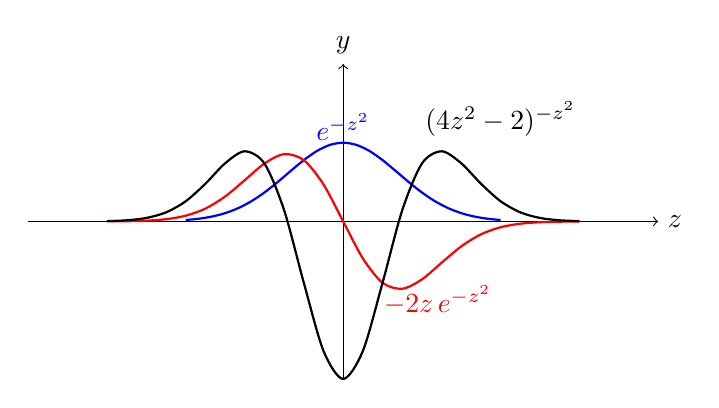
\begin{tikzpicture}
        \draw[->] (-4,0) -- (4,0) node[right] {$z$};
        \draw[->] (0,-2) -- (0,2) node[above] {$y$};
        \draw[domain=-2:2, smooth, variable=\x, blue, thick]
        plot({\x},{exp(-\x*\x)});
        \node[blue] at (0,1.2) {$e^{-z^2}$};

        \draw[domain=-3:3, smooth, variable=\x, red, thick, thick]
        plot ({\x}, {-2*\x*exp(-\x*\x)});
        \node[red] at (1.2,-1) {$-2z\,e^{-z^2}$};

        \draw[domain=-3:3, smooth, variable=\x, black, thick, thick]
        plot ({\x}, {(4*\x*\x - 2)*exp(-\x*\x)});
        \node[black] at (2,1.3) {$(4z^2-2)\ee^{-z^2}$};
    \end{tikzpicture}
    \caption{Diagram of Gaussian Function and the first, second order derivatives.}
    \label{fig:Gaussian}
\end{figure}

The first two orders of derivatives are 
\begin{align}
    G'(z) = - 2 z \ee^{-z^2} \\
    G''(z) = (4z^2-2) \ee^{-z^2}
\end{align}

The n-th order derivative is 
\begin{eqnarray}
    G^{(n)} (z) = (-1)^n H_n(z) \ee^{-z^2}
\end{eqnarray}
Where $H_n(z)$ is the n-th Polynomials of $z$. We can use Mathematical Induction to prove this, for $n=1,2$, the euqation above is obviously true, now we assume it holds for $n-1$ either, 
\begin{eqnarray}
    G^{(n-1)}(z) = (-1)^{n-1} H_{n-1} (z) \ee^{-z^2} 
\end{eqnarray}
Take derivative of this 
\begin{eqnarray}
    G^{(n)}(z) = (-1)^n \left(2z- \frac{\dd}{\dd z}\right) H_{n-1}(z) \ee^{-z^2}
\end{eqnarray}
We can find
\begin{eqnarray}
    H_n(z) = \left(2z-\frac{\dd}{\dd z}\right) H_{n-1}(z)
\end{eqnarray}
We can by this define \emph{Hermitian Polynomials}
\begin{eqnarray}
    H_n(z)=(-1)^n \mathrm{e}^{z^2} \frac{\mathrm{~d}^n}{\mathrm{~d} z^n} \mathrm{e}^{-z^2}
\end{eqnarray}

\newpage

































































































